% =====================================
% CAPÍTULO 2: ESTADO DEL ARTE Y MARCO TEÓRICO
% =====================================

\section{Estado del Arte y Marco Teórico}

\subsection{Estado del Arte}
    
El estudio de la adhesión fibra–matriz en materiales compuestos ha sido principalmente abordado
mediante ensayos a escala micromecánica, los cuales permiten caracterizar la resistencia
al corte interfacial (\textit{Interfacial Shear Strength}, IFSS) de fibras individuales embebidas
en una matriz polimérica. Entre los métodos más utilizados destacan el \textit{Single-Fiber Pull-Out
Test}, el \textit{Push-Out Test} y el \textit{Microdroplet Test} \cite{Miller1987, Gao2015, Ouyang2020}.
Estos ensayos han demostrado ser efectivos para estimar la fuerza de adhesión a nivel de un
filamento, pero presentan limitaciones importantes: alta dispersión de los resultados, baja
representatividad frente a la interacción colectiva de fibras, y dificultad para escalar
a configuraciones de ingeniería práctica \cite{DINSPEC19289, Liu2021}.

En años recientes, la \textbf{ISO 19375:2024} ha consolidado criterios para el \textit
{single-fibre pull-out} (control de alineación, geometría y reducción de datos), reforzando buenas
prácticas que pueden transferirse a otras configuraciones \cite{ISO19375}. En paralelo, varias
revisiones subrayan que la IFSS obtenida es una \textit{métrica aparente} sensible al estado de
tensiones no uniforme, al acoplamiento normal–corte y al modelo de reducción empleado; por ello,
se recomienda explicitar el procedimiento de cálculo y corroborar tendencias con métricas
complementarias cuando sea pertinente \cite{Fischer2020, Liu2021, AhmadvashAghbash2024IMR}.

Para superar estas limitaciones, se ha desarrollado el \textit{Fiber-Bundle Pull-Out Test}
(FBPO), que permite extraer hebras completas de fibras (aproximadamente 3000 filamentos por hebra)
embebidas en la matriz \cite{DeLeon2022}. Al trabajar en la mesoescala, este método captura
de manera más representativa la interacción colectiva fibra–matriz, reduciendo la dispersión de
los resultados y aumentando la robustez estadística. De León et al.\ describen un procedimiento
escalable basado en moldes multicavidad y dispositivos de alineación geométrica,
asegurando un control preciso de la longitud de embebido y permitiendo la producción repetible de
probetas homogéneas.

Adicionalmente, se ha mostrado que configuraciones FBPO mejoradas logran consistencia con
métodos micromecánicos (microbond/pull-out) y que la ruta de curado puede
reducir tiempos manteniendo o mejorando el desempeño interfacial, siempre que se controle el grado
de curado \cite{Zhou2016}. Para sistemas de fibras cortas y termoplásticos, estudios de \textit{push-out}
a microescala también han servido como referencia para entender cómo la “IFSS verdadera” puede diferir de
la aparente por distribuciones de tensión y confinamiento \cite{Liu2021}.

Además, la implementación de ensayos FBPO puede apoyarse en normativas existentes para fibras
individuales o hilos textiles, cuyas recomendaciones son transferibles a la mesoescala. La
\textbf{DIN SPEC 19289} establece procedimientos estandarizados para el \textit{single-fiber
pull-out}, enfatizando el control geométrico y la alineación durante el ensayo. La
\textbf{ISO 3341} proporciona lineamientos para la tracción de hilos de vidrio, incluyendo
prácticas de sujeción y acondicionamiento que pueden aplicarse a hebras completas. Por último,
la \textbf{DIN 29965} define especificaciones para hilos de carbono en aplicaciones aeroespaciales,
relevantes para la trazabilidad del material utilizado en probetas
\cite{DINSPEC19289, ISO3341, DIN29965}. La \textbf{ISO 19375:2024} aporta lineamientos adicionales de
alineación y validez para \textit{single-fibre pull-out}, útiles para inspirar configuraciones FBPO,
mientras que \textbf{ASTM D4475} muestra cómo se normalizan metodologías de corte/aparente en compuestos
pultruidos.

Más allá del montaje, la literatura enfatiza fuentes de variabilidad que afectan la comparación
entre estudios: (i) longitud embebida \(\ell_e\) y su dispersión real; (ii) velocidad de ensayo y
\emph{rate effects} sobre la fricción post–despegue; (iii) condición de superficie y \textit{sizing}
(química, espesor, energía superficial); y (iv) criterios de identificación de la carga de despegue
\(P^{\ast}\) y del área embebida efectiva \(A_e\) \cite{Fischer2020,Liu2021,AhmadvashAghbash2024IMR}.
Los estándares citados ofrecen listas de verificación transferibles al FBPO, las cuales permiten
reducir dispersión y mejorar trazabilidad mediante control de pretensión, bloqueo geométrico y reporte
sistemático de tolerancias.

A nivel histórico, el desarrollo de métodos experimentales para cuantificar la adhesión fibra–matriz
ha evolucionado desde los primeros microbond en los años 80, pasando por la consolidación del 
\textit{single-fibre pull-out} en los 90, el avance de técnicas ópticas/SEM/AFM en los 2000 y la 
incorporación de modelos shear–lag enriquecidos en la década de 2010. Desde 2015, los métodos 
mesoscópicos como FBPO se posicionan como alternativas más representativas para estudiar adhesión en 
hebras completas \cite{DeLeon2022}.

Los distintos ensayos aportan ventanas complementarias al fenómeno interfacial. El microbond 
representa despegue altamente localizado; el \textit{single-fibre pull-out} permite controlar \(\ell_e\); 
el \textit{push-out} revela efectos de confinamiento; y el FBPO introduce mecanismos colectivos de 
fricción y redistribución de carga. No existe equivalencia directa entre sus valores, ya que difieren 
sus estados tensionales, sensibilidad geométrica y escalas de medida.

El \textbf{sizing} emerge como el factor más determinante de la adhesión. A nivel químico regula la 
energía superficial y humectación; a nivel microestructural define rugosidad, espesor y continuidad de 
la capa; y en mesoescala controla la compactación del haz, el \textit{wicking} y la fricción colectiva. 
De León et al.\ demostraron mediante SEM/AFM que diferencias entre proveedores pueden modificar 
sistemáticamente los modos de falla y la fricción post–despegue \cite{DeLeon2022}.

El escalamiento micro→meso→macro es central para comprender la IFSS moderna: la micromecánica captura 
mecanismos locales; la mesomecánica (FBPO) captura efectos colectivos; y los ensayos estructurales 
permiten validar tendencias en configuraciones reales. En este sentido, FBPO actúa como un puente entre 
lo local y lo estructural, aportando valores más representativos que un filamento individual.

Finalmente, la variabilidad experimental sigue siendo un desafío. La literatura moderna recomienda 
un tratamiento estadístico explícito: ANOVA, intervalos de confianza, bloqueos por cavidad y 
verificación de supuestos. El FBPO, gracias a su naturaleza multicavidad, permite tamaños muestrales 
significativamente mayores que los ensayos micromecánicos tradicionales.

\subsubsection{Valores reportados en la literatura}

El \textit{review} más reciente sobre adhesión fibra–matriz \cite{AhmadvashAghbash2024IMR} compila
los rangos típicos de IFSS reportados para configuraciones micro, meso y macroscópicas en sistemas
carbono/epoxi y vidrio/epoxi. En general, los métodos micromecánicos presentan los valores más altos
debido al confinamiento geométrico y al estado tensional no uniforme, mientras que los métodos
mesoscópicos —como FBPO— entregan valores más moderados pero de mayor representatividad estadística.

% \begin{table}[htbp]
% \centering
% \caption{Rangos de IFSS reportados en la literatura para distintos métodos de ensayo.}
% \label{tab:ifss_rangos}
% \begin{tabular}{l c}
% \toprule
% \textbf{Método de ensayo} & \textbf{Rango de IFSS (MPa)} \\
% \midrule
% SFFT               & 30--100 \\
% Microbond          & 30--90  \\
% Push-Out / Push-In & 10--80  \\
% SFPO               & 20--50  \\
% FBPO               & 15--40  \\
% ILSS               & 40--80  \\
% Iosipescu          & 30--60  \\
% \bottomrule
% \end{tabular}
% \end{table}

Estos rangos reflejan claramente la disminución progresiva de la IFSS aparente al pasar de escalas
micromecánicas a mesoscópicas y finalmente a ensayos estructurales. La Fig.~\ref{fig:ifss_ranges} 
resume estos valores mediante un boxplot, lo que permite visualizar simultáneamente la amplitud del
rango reportado y las diferencias sistemáticas entre métodos. Este comportamiento coincide con lo
reportado por \cite{AhmadvashAghbash2024IMR}, quien destaca que los ensayos a microescala tienden a 
sobreestimar la adhesión debido a restricciones geométricas que no representan adecuadamente la 
interacción colectiva de una hebra completa.

% \begin{figure}[htbp]
%     \centering
%     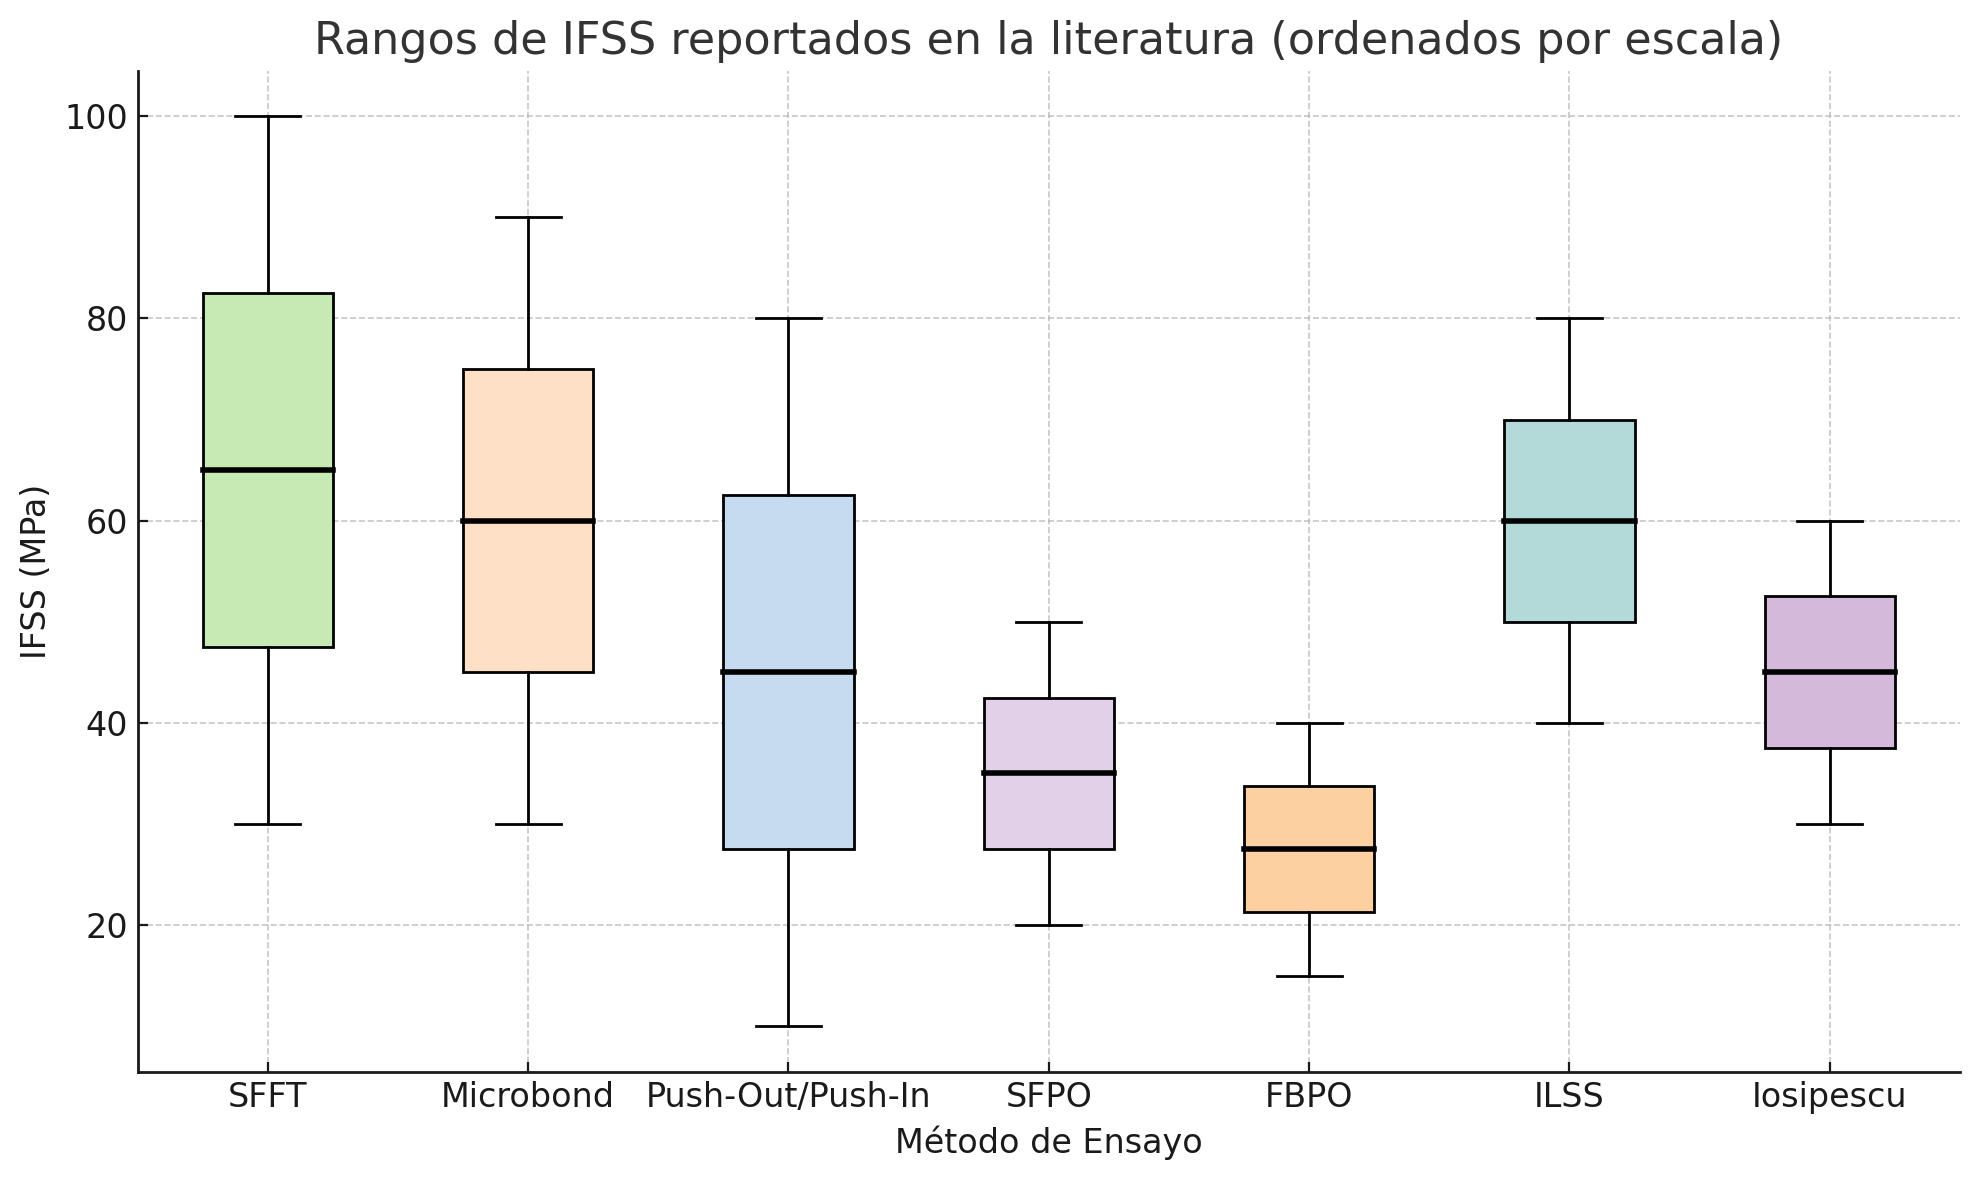
\includegraphics[width=0.85\linewidth]{IFSS_ranges_plot.png}
%     \captionsetup{justification=centering, singlelinecheck=false}
%     \caption{Rangos de IFSS reportados en la literatura para distintos métodos de ensayo.}
%     \label{fig:ifss_ranges}
% \end{figure}

\begin{figure}[htbp]
    \centering
    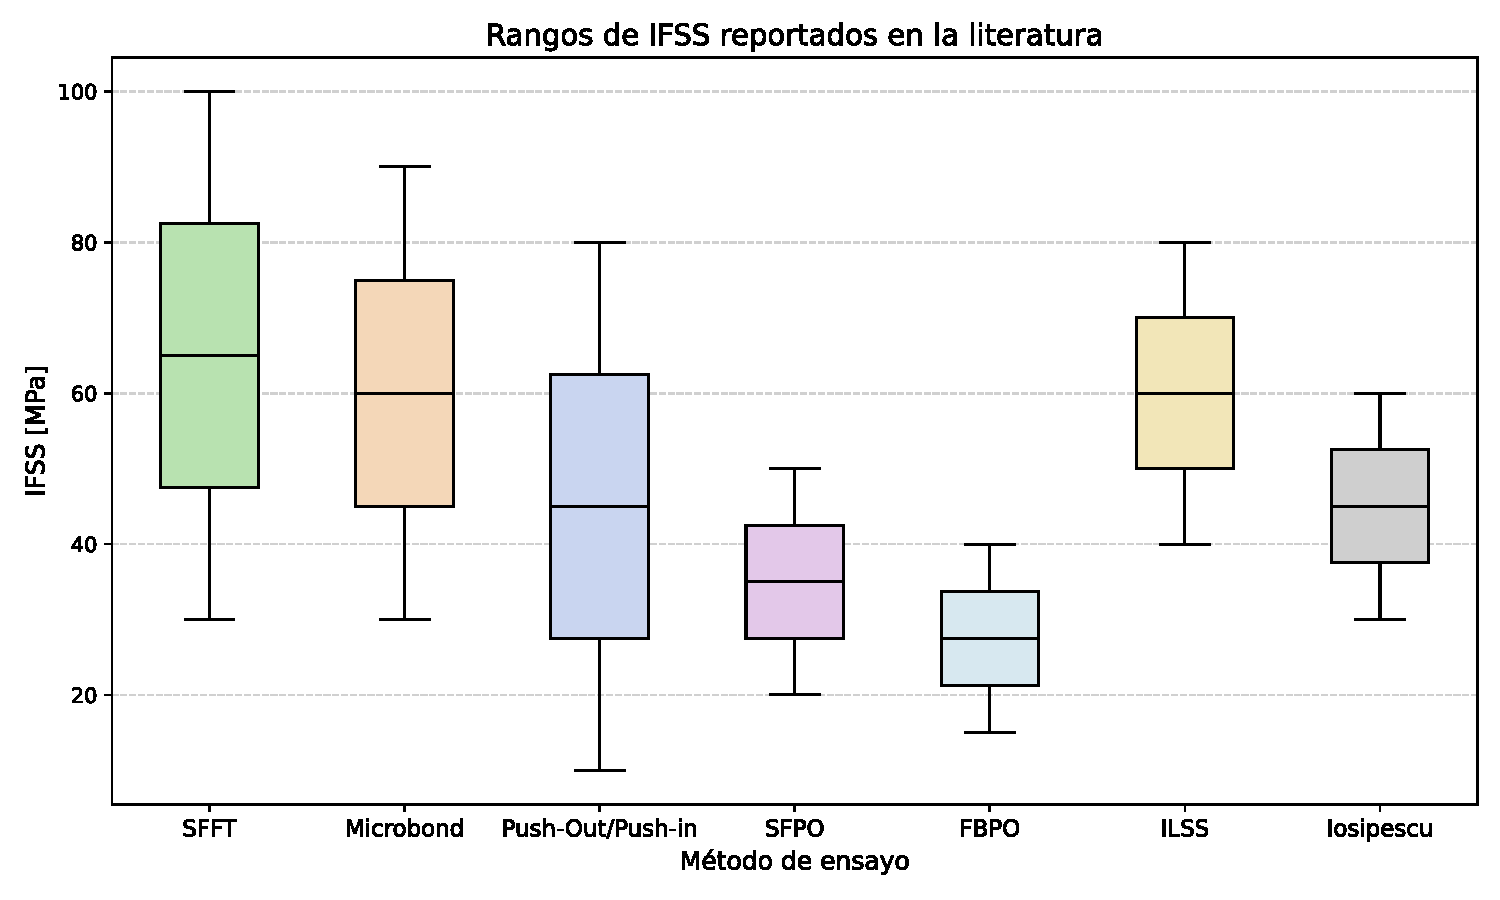
\includegraphics[width=0.85\linewidth]{IFSS_reportada_literatura}
    \captionsetup{justification=centering, singlelinecheck=false}
    \caption{Rangos de IFSS reportados para distintos métodos de ensayo \cite{AhmadvashAghbash2024IMR}.}
    \label{fig:ifss_ranges}
\end{figure}

% =======================================================
% ===================== DISCUSIÓN ========================
% =======================================================

\paragraph{Discusión.}

El FBPO se sitúa en una escala intermedia que permite reducir la elevada dispersión típica de los
ensayos micromecánicos convencionales sin perder sensibilidad hacia los mecanismos fundamentales de la
interfase. Sin embargo, la \(\tau_{\text{IFSS,ap}}\) obtenida continúa siendo un parámetro dependiente
del método, condicionado por el modelo de reducción empleado (\(P^{\ast}\)–\(A_e\)), la longitud embebida
\(\ell_e\), el perímetro efectivo \(d_{\mathrm{eq}}\) y la historia de procesamiento (curado, rugosidad,
\textit{sizing}). Los valores de FBPO no son directamente comparables con microbond, \textit{pull-out}
ni \textit{push-out}, pues cada método ilumina diferentes mecanismos interfaciales.

Esta dependencia refuerza la necesidad de interpretar resultados desde un enfoque multiescala: la
micromecánica captura fenómenos locales de adhesión, mientras que FBPO incorpora mecanismos colectivos
como fricción residual, redistribución de carga y variabilidad topológica del haz. A nivel estructural,
estas propiedades emergentes condicionan la tenacidad interlaminar y el desempeño transversal del
laminado.

El \textit{sizing} es uno de los factores más influyentes en la IFSS aparente. La evidencia de De León
et al.\ muestra que la morfología post–ensayo y la fricción residual permiten discriminar entre
interacciones interfaciales fuertes y débiles, imponiendo la necesidad de caracterizar superficie y
registrar lote/proveedor para aislar efectos reales.

La variabilidad experimental requiere un enfoque estadístico explícito: regresiones con intervalos de
confianza, análisis ANOVA, bloqueos por cavidad/lote y verificación de supuestos. El FBPO es especialmente
adecuado para esta aproximación debido a su escalabilidad y capacidad de generar grandes tamaños
muestrales.

Persisten brechas abiertas: ausencia de modelos universales que integren adhesión, fricción y topología
del haz; falta de criterios estandarizados para definir \(P^{\ast}\); y necesidad de profundizar en
modelos fisicoquímicos que describan el rol del \textit{sizing}. El presente trabajo replica y adapta la
metodología multicavidad propuesta por \cite{DeLeon2022} para comparar dos proveedores de la misma fibra
en idéntica resina, generando evidencia reproducible y trazable sobre la influencia del recubrimiento de
fábrica en la adhesión fibra–matriz a mesoescala.

%
% Marco teórico
%

\subsection{Marco Teórico}

El marco teórico tiene como objetivo proporcionar los conceptos fundamentales que sustentan la
implementación del ensayo \textit{Fiber-Bundle Pull-Out} (FBPO) y la interpretación de los
resultados obtenidos.

\subsubsection{Interfaz fibra – matriz}
La interfaz fibra – matriz se define como la región de contacto entre los filamentos de refuerzo y
la matriz polimérica en un material compuesto. Esta zona es crucial, ya que permite la
transferencia de esfuerzos desde la matriz hacia las fibras, determinando el comportamiento
mecánico global del material. La calidad de la interfaz influye directamente en la rigidez,
resistencia y tenacidad del compuesto, y un fallo en esta región puede conducir a una disminución
significativa de la vida útil de los componentes \cite{HullClyne1996, KellyZweben2000}.
Como se ilustra en la Fig~\ref{fig:interfaz_fibra_matriz}, el enlace interfacial puede
descomponerse en contribuciones químicas, mecánicas y friccionales, las cuales interactúan
entre sí y están fuertemente influenciadas por la química del \textit{sizing} y la historia de
procesamiento.

\begin{figure}[H]
    \centering
    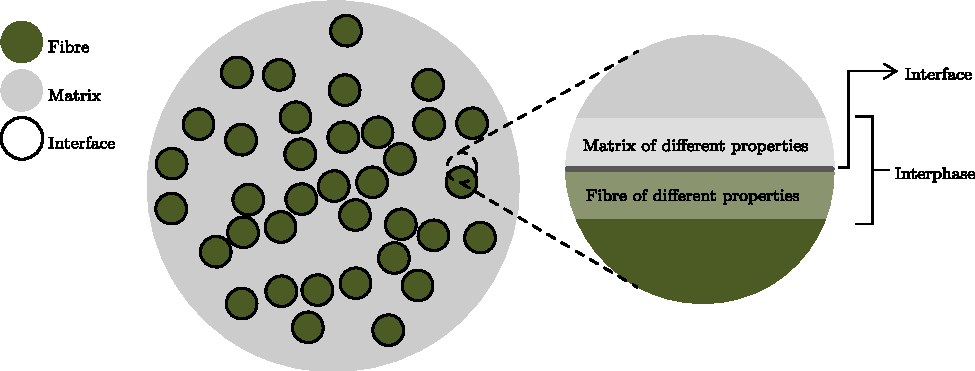
\includegraphics[width=0.75\linewidth]{interfaz.pdf}
    \captionsetup{justification=centering, singlelinecheck=false}
    \caption{Esquema representativo de la interfaz fibra–matriz en un material compuesto.}
    \label{fig:interfaz_fibra_matriz}
\end{figure}    

El enlace interfacial suele descomponerse en contribuciones químicas (compatibilidad entre grupos
funcionales de matriz y \textit{sizing}), anclaje mecánico (topografía/rugosidad efectiva) y fricción
post - despegue; estas contribuciones interactúan y pueden verse afectadas por tensiones residuales y
la historia de procesamiento (curado, contracción, etc) \cite{AhmadvashAghbash2024IMR, Liu2021}.
En términos microestructurales, puede existir una zona de interfase con gradientes de composición
y propiedades - influenciada por la química del \textit{sizing}, su espesor y la energía superficial -
que condiciona la iniciación del despegue y el modo de falla (cohesivo en matriz/interfase o adhesivo
en fibra) \cite{AhmadvashAghbash2024IMR,Liu2021}.

Operativamente, estas características se reflejan en la respuesta mecánica medida: la carga de
despegue \(P^{\ast}\) está fuertemente asociada a la tenacidad química/mecánica de la interfase,
mientras que el tramo post - despegue depende del confinamiento local y de la fricción fibra – matriz,
ambos sensibles al estado superficial y a la longitud embebida \(\ell_e\). Así, diferencias de
\textit{sizing} entre proveedores - aun con la misma fibra nominal y resina - pueden modificar el mojado,
la adhesión química y la fricción efectiva, alterando tanto la forma de la curva fuerza – desplazamiento
como la IFSS aparente estimada por reducción \(P^{\ast}\) – área \cite{Liu2021,AhmadvashAghbash2024IMR}.

\subsubsection{Resistencia al corte interfacial (IFSS)}
La \textit{Interfacial Shear Strength} (IFSS) describe la capacidad de la interfaz para resistir el
deslizamiento relativo entre fibra y matriz bajo solicitación de corte. Se estima habitualmente mediante
ensayos de tracción a escala micro o meso, entre los que destacan el \textit{single-fibre pull-out}, el
\textit{microbond} y, a mesoescala, el \textit{fiber-bundle pull-out} (FBPO) \cite{Gao2015,DeLeon2022}.
Su magnitud orienta el diseño y la optimización de compuestos, pues condiciona la transferencia de carga
y, en consecuencia, la respuesta mecánica global.

En el caso de FBPO, la IFSS reportada se considera una medida \emph{aparente}: depende del modelo de
reducción adoptado para convertir la señal fuerza – desplazamiento en un parámetro de adhesión y del estado
real de tensiones en la interfase. La práctica recomendada en la literatura consiste en identificar el
punto de despegue en la curva experimental, relacionarlo con la extensión de contacto fibra – matriz y
obtener una pendiente representativa del nivel de adhesión, siempre informando el procedimiento de
cálculo, los supuestos asumidos y la incertidumbre asociada \cite{Fischer2020,Liu2021,DeLeon2022}.
Este enfoque privilegia la comparación de tendencias entre condiciones controladas antes que la
equivalencia numérica con otros métodos.

La IFSS es sensible a variables geométricas (longitud embebida, compactación de la hebra), de ejecución
(alineación, velocidad de ensayo), de proceso (ruta y grado de curado, tensiones residuales) y de
superficie (química y espesor del \textit{sizing}, rugosidad efectiva). También influye el criterio
operativo para identificar el despegue y la calidad de la sujeción. Por ello, se aconseja normalizar
la preparación y el reporte con lineamientos de alineación, geometría, sujeción y validez, y respaldar
la interpretación con métricas complementarias cuando sea pertinente
\cite{ISO19375,Fischer2020,Liu2021,Zhou2016}. Bajo estas premisas, la IFSS aparente se convierte en un
indicador robusto para juzgar diferencias de adhesión entre materiales o tratamientos, manteniendo
explícito su carácter dependiente del modelo y de las condiciones de ensayo.

\subsubsection{IFSS aparente vs.\ real}

La resistencia al corte interfacial reportada en los ensayos (IFSS) es, en la mayoría de los casos,
una \emph{magnitud aparente}. Esto se debe a que su cálculo se basa en modelos de reducción que
suponen condiciones idealizadas: distribución uniforme de corte, perímetro constante, ausencia de
tensiones normales y contacto perfecto fibra–matriz. En configuraciones reales, estos supuestos no se
cumplen estrictamente debido a fenómenos como rugosidad superficial, gradientes de adherencia,
infiltración capilar (\textit{wicking}), fricción post–despegue y heterogeneidad en la compactación del
haz \cite{Liu2021,AhmadvashAghbash2024IMR}.

Por ello, la IFSS calculada representa una combinación efectiva de adhesión química, anclaje
mecánico y fricción residual. Su valor depende del método utilizado (microbond, pull-out,
push-out, FBPO), de la escala del ensayo y del modelo adoptado para interpretar la curva
fuerza–desplazamiento. En este contexto, la comparación de IFSS entre distintos métodos no debe
realizarse en términos absolutos, sino interpretando \emph{tendencias bajo condiciones controladas} y
especificando siempre el modelo y supuestos utilizados en la reducción de datos.

\subsubsection{Mecanismos de falla interfacial}

El despegue fibra–matriz puede involucrar diversos mecanismos que se manifiestan de forma secuencial
o simultánea:

\begin{itemize}
    \item \textbf{Falla adhesiva:} ocurre en la superficie de la fibra cuando la química del
    \textit{sizing} o la humectación son insuficientes. La carga cae abruptamente al perderse el
    anclaje químico inicial.

    \item \textbf{Falla cohesiva en la interfase:} el desgarro se produce en una capa interfacial
    modificada (zona rica en \textit{sizing}, regiones con reticulación parcial o gradientes
    fisicoquímicos). Este mecanismo indica la presencia de una ``zona de transición'' entre fibra y
    matriz.

    \item \textbf{Falla cohesiva en la matriz:} la grieta se propaga dentro de la resina adyacente,
    típica de matrices frágiles o con tensiones residuales elevadas. Puede aumentar la carga de
    despegue aparente aun cuando la adhesión no sea alta.

    \item \textbf{Deslizamiento friccional post–despegue:} tras la pérdida de anclaje químico,
    la interacción está dominada por presión normal, rugosidad superficial y compactación del haz. La
    fricción puede contribuir significativamente a la carga medida, especialmente en FBPO donde miles
    de filamentos participan colectivamente \cite{DeLeon2022}.
\end{itemize}

La curva fuerza–desplazamiento permite identificar estos mecanismos: una pendiente inicial asociada
a la adhesión, un punto de despegue \(P^{\ast}\), una caída abrupta y un régimen posterior dominado por
fricción. La coexistencia de mecanismos explica por qué la IFSS aparente no representa estrictamente
una propiedad intrínseca del material, sino una respuesta efectiva del sistema fibra–interfase–matriz.

\subsubsection{Escalas de estudio}
\begin{itemize}
    \item \textbf{Micromecánica:} Se centra en un \emph{filamento individual} embebido en matriz y
	utiliza montajes de alta precisión (pull-out de un solo filamento, \textit{microbond},
	\textit{push-out}). Entrega métricas de adhesión locales (IFSS) con alto control de variables
	químicas (tipo de \textit{sizing}, funcionalización) y geométricas a microescala
	\cite{Miller1987,Ouyang2020}. Sus \emph{ventajas} son el aislamiento del mecanismo interfacial
	y la sensibilidad a cambios finos de superficie; sus \emph{limitaciones} incluyen alta dispersión,
	efectos de borde, daño por sujeción y baja representatividad del comportamiento colectivo de una
	hebra. Es muy sensible a la alineación, a la longitud embebida y al criterio de identificación del
	despegue; por ello se beneficia de lineamientos como \cite{ISO19375,DINSPEC19289} para control
	geométrico, reducción de datos y validez de muestras. Resulta idónea para \emph{cribado} de
	recubrimientos y estudios mecanísticos de química de interfase.

\begin{figure}[H]
    \centering
    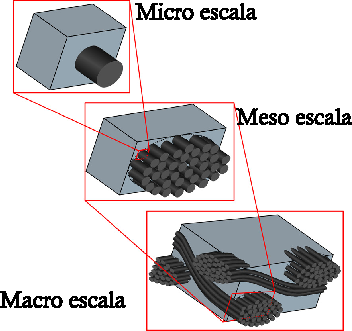
\includegraphics[width=0.4\linewidth]{escalas_de_estudio.pdf}
    \captionsetup{justification=centering, singlelinecheck=false}
    \caption{Escalas de compuesto tejido de fibra.}
    \label{fig:escalas_de_estudio}
\end{figure} 

    \item \textbf{Mesoescala:} Considera una \emph{hebra completa} (típicamente \(\sim\)3000 filamentos)
	embebida en matriz y representa la interacción \emph{colectiva} fibra – matriz \cite{DeLeon2022}.
	El \textit{Fiber-Bundle Pull-Out} (FBPO) permite reducir la dispersión y mejorar la robustez
	estadística respecto de la micromecánica, a la vez que mantiene sensibilidad a la interfase
	(química del \textit{sizing}, mojado y fricción post-despegue). Sus \emph{ventajas} son la mayor
	representatividad y la posibilidad de \emph{escalar la fabricación} de probetas (molde multicavidad)
	para análisis con potencia estadística; sus \emph{desafíos} son el estado de tensiones complejo y la
	necesidad de un modelo de reducción explícito (IFSS \emph{aparente}) con buena metrología de
	longitud embebida y diámetro equivalente de la hebra \cite{Fischer2020,Liu2021}. Es especialmente
	útil para comparar proveedores de la misma fibra y resina, evaluar efectos de proceso/curado y
	generar datos transferibles a niveles superiores \cite{DeLeon2022}.

    \item \textbf{Macroscópica:} Analiza \emph{laminados o componentes} completos donde interactúan
	arquitectura de apilamiento, volumen de fibra, geometría y condiciones de carga reales. Métodos
	habituales: Iosipescu (corte), ILSS/short-beam, tracción \(\pm45^\circ\), flexión; los resultados
	integran mecanismos múltiples (matriz, interfaz, arquitectura) y reflejan relevancia de ingeniería.
	Sus \emph{ventajas} son la aplicabilidad directa y la posibilidad de validar tendencias observadas
	en micro/meso; sus \emph{limitaciones} incluyen la no unicidad del mecanismo de falla y la
	dificultad para atribuir cambios exclusivamente a la interfase. Es apropiada para
	\emph{verificación de coherencia} con FBPO y para estudiar el impacto neto de modificaciones de
	interfase en el desempeño estructural global \cite{Liu2021,Fischer2020}.
\end{itemize}

\subsubsection{Variables experimentales que afectan la IFSS}
\begin{itemize}
    \item \textbf{Alineación axial (coaxialidad hebra–carga).} 
    Foco en mantener el eje de la hebra coincidente con la línea de carga para evitar momentos y tensiones
	normales parásitas. Desalineaciones alteran el umbral de despegue y la fricción post – despegue,
	elevando la dispersión. Control típico: guiado geométrico del molde/fixture, superficies de
	referencia paralelas, pretensión mínima y verificación visual; seguir lineamientos de
	alineación/validez \cite{ISO19375,DINSPEC19289}.

    \item \textbf{Longitud embebida (\(\ell_e\)).} 
    Determina la extensión efectiva de contacto fibra–matriz; su variación impacta directamente la carga
	de despegue y la pendiente usada para estimar la IFSS aparente. Se controla con topes en el molde y
	se verifica en probetas testigo (inspección óptica); conviene registrar por cavidad para permitir
	“bloqueo por cavidad” en el análisis \cite{DeLeon2022}. Recomendación: fijar tolerancias explícitas
	y descartar probetas fuera de especificación.

    \item \textbf{Velocidad de ensayo (tasa de desplazamiento).} 
    Afecta la detección del despegue y la magnitud de la fricción post – despegue (\emph{rate effects}). 
    Debe mantenerse constante dentro de un lote y reportarse con su tolerancia; evitar mezclar tasas en
	comparaciones directas. Verificación previa con corrida en vacío y registro de la tasa real de la
	máquina \cite{ISO19375,Fischer2020,Liu2021}.

    \item \textbf{Criterio de \emph{muestra válida}.} 
    Define las condiciones mínimas para aceptar un resultado (p.\,ej., extracción completa de la hebra,
	sin deslizamiento en mordazas ni daño del bloque, señal fuerza – desplazamiento sin artefactos). Debe
	declararse antes de la campaña, junto con causas de descarte y evidencias (fotos/notas). Esto mejora
	la comparabilidad interlaboratorio y reduce sesgos de selección \cite{ISO19375,DINSPEC19289}.
\end{itemize}

\noindent
La estandarización y el reporte explícito de estas variables - incluidas sus tolerancias y criterios de
aceptación - son esenciales para reducir la dispersión, habilitar análisis estadísticos robustos y
facilitar la comparación entre estudios \cite{ISO19375,DINSPEC19289,Fischer2020,Liu2021}.

\subsubsection{Ensayos de caracterización interfacial}
Los ensayos más utilizados para la medición de IFSS incluyen Fig~\ref{fig:tipos_de_ensayos}:

\begin{figure}[H]
    \centering
    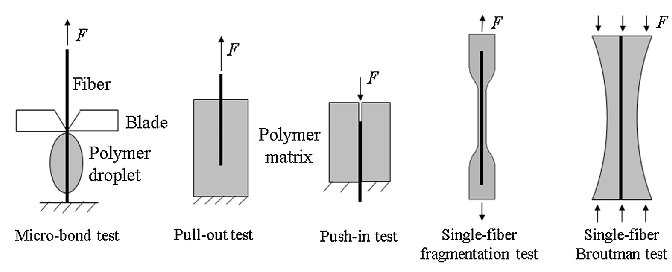
\includegraphics[width=0.75\linewidth]{tipos_de_ensayos.pdf}
    \captionsetup{justification=centering, singlelinecheck=false}
    \caption{Tipos de ensayo a microescala.}
    \label{fig:tipos_de_ensayos}
\end{figure}

\begin{itemize}
    \item \textbf{\textit{Single-Fiber Pull-Out Test:}} Evalúa la adhesión extrayendo un único filamento
	previamente embebido en una microresina o matriz, con control fino de la longitud de embebido y de
	la alineación axial. Su principal fortaleza es el acceso directo al fenómeno interfacial y la
	sensibilidad a cambios de superficie/sizing; sin embargo, presenta alta dispersión de resultados
	por daño de sujeción, variaciones geométricas a microescala y sensibilidad a la identificación del
	despegue. Requiere una reducción cuidadosa de datos y criterios de validez rigurosos, para lo cual
	las guías más recientes ayudan a estandarizar alineación, geometría y reporte
	\cite{Miller1987,ISO19375,DINSPEC19289}.

    \item \textbf{\textit{Push-Out Test:}} Determina la resistencia interfacial empujando la fibra hacia
    fuera desde una microsección pulida del compuesto mediante un indentador controlado, mientras se
	monitoriza la fuerza de expulsión. Se utiliza principalmente en composites de alta precisión o en
	estudios donde se busca minimizar artefactos de sujeción del filamento, permitiendo análisis
	locales e incluso mapeo espacial de la interfase. Entre sus limitaciones se encuentran la preparación
	de muestras (sección delgada, pulido controlado), la influencia del confinamiento circundante y
	la dificultad de extrapolar los resultados a condiciones de tracción a escala mayor \cite{Ouyang2020}.

    \item \textbf{\textit{Microdroplet Test:}} Consiste en depositar microgotas de matriz sobre fibras
	individuales y medir la fuerza necesaria para deslizar o arrancar la gota, relacionándola con
	la longitud mojada. Es un método ágil para cribar formulaciones de resina o tratamientos
	superficiales, con requisitos de utillaje relativamente bajos. Sus principales desafíos son la
	reproducibilidad de la geometría de las gotas, la correcta medición de la longitud mojada y el
	control de artefactos por tensión superficial o curvatura de la fibra; como en otros ensayos
	micromecánicos, la dispersión puede ser elevada y la representatividad frente a hebras completas
	es limitada \cite{Gao2015,Ouyang2020}.

    \item \textbf{\textit{Fiber-Bundle Pull-Out Test (FBPO):}} Extrae una hebra completa (típicamente miles
    de filamentos) parcialmente embebida en la matriz, capturando la interacción colectiva fibra – matriz.
	Esta configuración reduce la dispersión típica de la micromecánica, mejora la robustez estadística
	y permite estudiar efectos de proceso y de \textit{sizing} con mayor representatividad. Sus retos
	incluyen el estado de tensiones más complejo, la necesidad de un modelo de reducción explícito
	(IFSS aparente) y una metrología cuidadosa de la longitud embebida y del diámetro equivalente de
	la hebra. El uso de moldes multicavidad y alineación geométrica, tal como propone \cite{DeLeon2022},
	facilita escalabilidad, trazabilidad y comparabilidad entre lotes \cite{DeLeon2022,Liu2021}.
\end{itemize}

En la práctica, la comparación cruzada entre métodos (p.\,ej., FBPO vs.\ microbond/pull-out) puede
mostrar coherencia de tendencias si se controlan las condiciones de fabricación y de ensayo; no obstante,
las magnitudes no son directamente intercambiables por las diferencias en estado de tensiones y escala
de medida \cite{Zhou2016, Fischer2020}. En consecuencia, se recomienda limitar el análisis a la
dirección y tamaño relativo de los efectos (p.\,ej., impacto del \textit{sizing} o del curado) bajo
protocolos armonizados de alineación, geometría, velocidad y criterios de validez
\cite{ISO19375,DINSPEC19289}, reportando la incertidumbre (intervalos de confianza) y aplicando ANOVA
con bloqueo cuando existan fuentes sistemáticas (cavidad, lote) \cite{Fischer2020,Liu2021}. La validez
externa puede reforzarse corroborando tendencias con métricas complementarias a otra escala (p.\,ej.,
ILSS o Iosipescu) y con configuraciones FBPO escalables y trazables (molde multicavidad, control
metrológico de \(\ell_e\)) que facilitan la repetibilidad interlote \cite{DeLeon2022}.

\subsubsection{Efecto del \textit{sizing} y la topografía superficial}
Diferencias en el recubrimiento de fábrica (\textit{sizing}) entre proveedores pueden modificar el mojado
inicial, la compatibilidad química con la matriz (p.\,ej., agentes de acoplamiento y grupos funcionales
reactivos) y el anclaje mecánico a través de la topografía efectiva; estas variables inciden en la
nucleación del despegue y en la fricción post – despegue, alterando la IFSS aparente y la morfología de
la curva fuerza – desplazamiento \cite{AhmadvashAghbash2024IMR,Liu2021}. El espesor y la continuidad del
\textit{sizing}, su estado de curado, posibles migraciones durante el curado de la matriz y la
presencia de plastificantes o contaminantes superficiales impactan la energía superficial y las
tensiones residuales locales. A nivel del haz, la compactación y el \emph{spreading} de filamentos
(grado de apertura/cierre), así como defectos locales (microdaños, contaminación) condicionan la
uniformidad de la transferencia de carga y, por ende, la dispersión de \(P^{\ast}\) y del tramo de
fricción \cite{Fischer2020}. La rugosidad efectiva—derivada de tratamientos oxidativos, plasma o
variaciones de trenzado/encolado—puede incrementar la presión normal efectiva y la fricción, desplazando
el equilibrio adhesión–fricción y modificando los modos de falla.

Para relacionar cambios de interfase con variaciones de adhesión se recurre a caracterizaciones
complementarias: AFM (rugosidad y módulo local), SEM/EDS (morfología y elementos), FTIR/XPS (química
de superficie), ángulo de contacto/energía superficial (mojado) y, cuando es viable, DSC/DMTA
(historia térmica y grado de curado) \cite{AhmadvashAghbash2024IMR,Liu2021}. En FBPO, se recomienda
documentar lote y proveedor, protocolo de acondicionamiento, historial térmico y mediciones básicas
de la hebra (masa lineal, diámetro equivalente), además de establecer criterios de \emph{muestra válida}
y un plan estadístico (ANOVA con bloqueo por cavidad/lote) para discernir efectos de \textit{sizing}
de artefactos de montaje \cite{Fischer2020,ISO19375}. Este enfoque permite interpretar la IFSS
aparente como un indicador reproducible de tendencias, manteniendo explícita su dependencia del
modelo de reducción y de las condiciones superficiales y de proceso.

\subsubsection{Profundización en el rol del \textit{sizing}}

El \textit{sizing} —el recubrimiento superficial industrial aplicado a las fibras— es uno de los
factores más influyentes en la adhesión fibra–matriz. Su función principal es compatibilizar la
superficie de la fibra con la química de la matriz y proteger los filamentos durante el manejo; sin
embargo, su impacto en la IFSS proviene de múltiples niveles:

\begin{itemize}
    \item \textbf{Nivel químico:} grupos funcionales específicos promueven la humectación y la
    reactividad con la matriz (p.\,ej., agentes de acoplamiento en sistemas epoxi). Diferencias
    entre proveedores pueden modificar la polaridad, energía superficial y densidad de sitios
    reactivos \cite{AhmadvashAghbash2024IMR}.

    \item \textbf{Nivel microestructural:} el espesor, continuidad y estado de curado del
    \textit{sizing} afectan la formación de una zona interfacial homogénea. Capas demasiado gruesas,
    incompletas o parcialmente curadas pueden alimentar fallas cohesivas o transiciones frágiles.

    \item \textbf{Nivel mesoscópico (hebra completa):} el \textit{sizing} regula el mojado entre
    filamentos, la compactación del haz, la formación de microcanales y la fricción colectiva. Estas
    variables influyen directamente en el comportamiento del FBPO, donde la interacción colectiva
    determina la pendiente \(P^{\ast}\)–\(A_e\) y el régimen friccional post–despegue
    \cite{DeLeon2022}.

    \item \textbf{Nivel macroscópico:} diferencias de \textit{sizing} se traducen en variaciones de
    ILSS, resistencia transversal, disipación de energía y durabilidad. Ensayos FBPO permiten anticipar
    tendencias de estas propiedades sin requerir tamaños muestrales grandes.
\end{itemize}

Pequeñas variaciones en formulaciones nominalmente similares pueden producir cambios sistemáticos en
el modo de falla, la fricción post–despegue y la morfología observada por SEM/AFM. Por ello, la
comparación entre proveedores requiere un control estricto de condiciones superficiales, ambientales y
procesos de curado para aislar el efecto real del \textit{sizing}.

% \subsubsection{Criterio de \emph{muestra válida}}
% \begin{itemize}
%   \item \textbf{Integridad del evento de extracción.}
%   La hebra debe extraerse completamente del bloque sin fractura del haz previa al despegue ni daño del
%   bloque/mordazas. Señales de deslizamiento o rotación del bloque invalidan el ensayo
%   \cite{ISO19375,DINSPEC19289}.

%   \item \textbf{Calidad de la señal fuerza–desplazamiento.}
%   Línea base estable, resolución suficiente y \emph{identificación clara} del despegue; ausencia de
%   saturaciones, pérdidas de dato o artefactos eléctricos. Se registra \emph{preload} y tasa nominal.

%   \item \textbf{Conformidad geométrica.}
%   Longitud embebida dentro de tolerancias y hebra sin daño visible ni nudos; alineación axial con la
%   línea de carga (coaxialidad). Se aconseja verificación metrológica en probetas testigo
%   \cite{ISO19375,DINSPEC19289}.

%   \item \textbf{Condiciones de ejecución.}
%   Velocidad de ensayo constante dentro de tolerancia; ambiencia (T/HR) registrada y dentro de rango;
%   protocolo de sujeción reproducible (protección antiaplastamiento).

%   \item \textbf{Trazabilidad y descarte.}
%   Identificación unívoca (proveedor, lote, cavidad, fecha) y evidencia de descarte (foto/notas)
%   cuando procede. Criterios predefinidos para evitar sesgo de selección \cite{ISO19375,DINSPEC19289}.
% \end{itemize}

\subsubsection{Análisis estadístico (normalidad, ANOVA y Tukey)}
\begin{itemize}
  \item \textbf{Supuestos y pruebas previas.}
  Antes de comparar grupos se verifican los supuestos básicos: que los datos de cada grupo sigan una
  distribución aproximadamente normal (prueba de Shapiro – Wilk) y que las varianzas sean similares entre
  grupos (Levene o Brown – Forsythe). Si alguno falla, se pueden aplicar transformaciones sencillas de
  los datos o recurrir a métodos no paramétricos. Además, se garantiza la independencia por diseño y,
  cuando existe estructura experimental (p.\,ej., cavidades o lotes), se incorpora como factor de
  \emph{bloqueo} para controlar variaciones ajenas al efecto principal \cite{Fischer2020,Liu2021}.

  \item \textbf{ANOVA (efecto global).}
  El ANOVA de un factor permite evaluar si las medias de los grupos (p.\,ej., proveedores o condiciones)
  difieren más de lo esperable por azar, siempre que se cumplan los supuestos previos. Se reportan el
  estadístico \(F\), el valor \(p\), intervalos de confianza y una medida del tamaño del efecto para
  interpretar la relevancia práctica. Si las varianzas son desiguales, se utiliza la versión de Welch.
  Cuando hay fuentes conocidas de variación sistemática, el ANOVA con \emph{bloqueo} reduce el error
  residual y mejora la sensibilidad del contraste \cite{Liu2021}.

  \item \textbf{Comparaciones múltiples (Tukey).}
  Si el efecto global resulta significativo, se aplican comparaciones post hoc para identificar qué pares
  de grupos difieren entre sí. La prueba de Tukey HSD controla el error por realizar múltiples
  comparaciones y ofrece diferencias de medias con sus intervalos y valores \(p\) ajustados. En
  escenarios con varianzas desiguales o tamaños muestrales distintos, es preferible usar Games – Howell.
  En todos los casos, se mantiene consistencia de las condiciones experimentales entre grupos para
  asegurar comparaciones válidas.

  \item \textbf{Incertidumbre y alternativas.}
  La estimación de la incertidumbre se refuerza mediante intervalos de confianza y, cuando el tamaño
  muestral es moderado o la distribución se aparta de la normalidad, con procedimientos de
  \emph{bootstrap}. Si los supuestos paramétricos no se satisfacen de forma persistente, se emplean
  alternativas como Kruskal – Wallis para el contraste global y la prueba de Dunn (con
  ajuste) para comparaciones por pares \cite{Fischer2020}.

  \item \textbf{Salida mínima y transparencia.}
  El reporte debe incluir, para cada grupo, el número de muestras válidas, medidas de tendencia central
  y dispersión, y representaciones gráficas simples. Para el contraste, se informan el resultado del
  test global, las comparaciones post hoc con intervalos de confianza, el tamaño del efecto y cualquier
  factor de \emph{bloqueo} considerado. Las exclusiones se documentan conforme al criterio de
  muestra válida, asegurando trazabilidad y reproducibilidad \cite{ISO19375,DINSPEC19289,Liu2021}.
\end{itemize}

\subsubsection{Normas y estandarización}
La realización de ensayos de adhesión se respalda en normas técnicas, que aseguran la
reproducibilidad y trazabilidad de los resultados. Entre ellas destacan:
\begin{itemize}
    \item \textbf{DIN SPEC 19289.} Establece un procedimiento para el \textit{single-fiber pull-out}
	con énfasis en la alineación axial, el control geométrico de la longitud embebida y la calidad de
	la señal fuerza–desplazamiento. Define criterios de validez, prácticas de sujeción y recomendaciones
	para la reducción de datos, con el objetivo de minimizar fuentes comunes de dispersión y sesgo
	\cite{DINSPEC19289}. 

    Asimismo, promueve la trazabilidad mediante el registro de lotes, condiciones ambientales y
	parámetros de ejecución (velocidad, pretensión, resolución de medición). Estas pautas, aunque
	concebidas para un único filamento, resultan transferibles a montajes a mesoescala como FBPO al
	estructurar listas de verificación (alineación, tolerancias, descarte) y al estandarizar el reporte.

    \item \textbf{ISO 3341.} Norma enfocada en la determinación de la fuerza de ruptura y la elongación
	de hilos de vidrio, con prácticas de acondicionamiento (temperatura y humedad), sujeción y tasa de
	carga reproducibles. Su interés para este trabajo radica en la unidad de ensayo (hebra) y en la
	armonización de procedimientos que evitan daño por mordazas o efectos de borde \cite{ISO3341}. 

    En el contexto FBPO, estas directrices aportan criterios operativos para el manejo de hebras:
	pretensión controlada, identificación de probetas, y consistencia de la tasa de ensayo. Contribuyen,
	además, a la comparabilidad interlote e interlaboratorio al fijar condiciones ambientales y de
	preparación previas al ensayo.

    \item \textbf{DIN 29965.} Reúne especificaciones para hilos de carbono en aplicaciones aeroespaciales,
	tales como designaciones, masas lineales, requisitos de calidad y métodos de verificación. Si bien
	no prescribe un ensayo de adhesión, fortalece la trazabilidad del material al definir parámetros
	nominales y tolerancias asociadas al hilo \cite{DIN29965}. 

    Para FBPO, estas especificaciones sustentan la documentación de proveedores y lotes, y sirven de
	base para comparar materiales “nominalmente iguales” pero con posibles diferencias de \textit{sizing}
	o acabado superficial. En conjunto, refuerzan la consistencia del muestreo y la interpretación de
	diferencias en IFSS aparente.

    \item \textbf{ISO 19375:2024.} Estandariza el \textit{single-fibre pull-out} con criterios modernos
	de control geométrico, alineación y reducción de datos. Incluye recomendaciones explícitas sobre
	la declaración de supuestos y la comunicación del carácter “aparente” de la IFSS bajo el modelo
	adoptado \cite{ISO19375}. 

    Su valor en FBPO es doble: ofrece un marco claro para definir tolerancias y validez del ensayo
	(alineación, identificación del despegue, calidad de señal) y facilita adaptar prácticas de reporte
	(incertidumbre, criterios de descarte) a una configuración de hebra, mejorando la comparabilidad
	de resultados entre escalas.

    \item \textbf{ASTM D4475.} Proporciona un referente de normalización para métodos de corte/
	aparente en materiales pultruidos, detallando apartados de aparejos, calibración, tasa de carga y
	reporte. Aunque no trata un \textit{pull-out} polimérico, su estructura metodológica es útil para
	discutir escalas de medida y control de variables en ensayos de extracción \cite{ASTMD4475}. 

    Trasladado a FBPO, su enfoque fomenta especificar con claridad los dispositivos de sujeción,
	las verificaciones de equipo, las tolerancias de velocidad y los criterios de salida (datos
	válidos/post hoc). De este modo, sirve como guía complementaria para fortalecer la calidad
	metrológica y la transparencia del informe técnico.
\end{itemize}

En síntesis, la adhesión fibra – matriz se entiende como un fenómeno multiescala que integra
química de superficie, anclaje mecánico y fricción post – despegue, cuya manifestación depende del
método de ensayo y del modelo de reducción adoptado. La IFSS debe interpretarse como una magnitud
operativa - frecuentemente aparente - condicionada por la geometría efectiva de contacto, el estado
de tensiones y las variables de ejecución. Bajo este prisma, los ensayos micromecánicos ofrecen
sensibilidad a la interfase, los de mesoescala (FBPO) añaden representatividad y robustez estadística,
y los macroscópicos permiten verificar coherencia de tendencias en configuraciones estructurales.

La implementación del FBPO se beneficia de lineamientos normativos concebidos para filamento único o
para hilos, que son transferibles a la mesoescala: control de alineación y geometría, sujeción
reproducible, acondicionamiento y criterios de validez \cite{ISO19375,DINSPEC19289,ISO3341,DIN29965}.
En particular, la metodología de \cite{DeLeon2022} - molde multicavidad y referencias metrológicas de
longitud embebida - habilita campañas con mayor tamaño muestral y reducción de datos consistente
(pendiente de despegue frente a área embebida), mientras que \cite{ASTMD4475} aporta una estructura de
reporte y control de variables útil para estandarizar ensayos de extracción en general.

La calidad inferencial de los resultados depende del control explícito de variables críticas
(alineación, \(\ell_e\), velocidad, criterio de muestra válida) y de un plan estadístico acorde:
verificación de supuestos, ANOVA (con Welch o bloqueo cuando corresponda), comparaciones post hoc
(Tukey/Games - Howell) y estimación de incertidumbre mediante intervalos de confianza y, si es necesario,
\emph{bootstrap} \cite{Fischer2020,Liu2021}. Complementariamente, la caracterización de superficie
(AFM/SEM/FTIR) permite vincular cambios de interfase con variaciones de IFSS, especialmente
relevante cuando se estudian diferencias de \textit{sizing} entre proveedores
\cite{AhmadvashAghbash2024IMR}. La coherencia externa puede reforzarse contrastando tendencias con
métricas a otras escalas (ILSS o Iosipescu) y verificando el grado de curado cuando se
modifican rutas de procesado \cite{Zhou2016}.

En este contexto, el presente trabajo replica y adapta la estrategia de \cite{DeLeon2022} para
evaluar, en una misma resina y con la misma fibra nominal, el efecto del \textit{sizing} de dos
proveedores sobre la IFSS aparente a mesoescala. El conjunto de criterios normativos y metodológicos
citados sustenta la trazabilidad, la comparabilidad interlote y la interpretación prudente de
resultados, asegurando que las conclusiones reflejen diferencias materiales y no artefactos de montaje
o de reducción. Este marco teórico, por tanto, no solo fundamenta la metodología propuesta, sino que
delimita su alcance y sus limitaciones, orientando el análisis hacia evidencias reproducibles y
útiles para el diseño de materiales compuestos.